\documentclass[../main/main.tex]{subfiles}
\begin{document}

\section{Basic Design Patterns}

The following graphics come from the official Wikipedia pages (German and English): 

\begin{itemize}
\item http://de.wikipedia.org/wiki/Strategie_%28Entwurfsmuster%29
\item http://en.wikipedia.org/wiki/Factory_method_pattern
\item http://en.wikipedia.org/wiki/Observer_pattern
\item http://en.wikipedia.org/wiki/Singleton_pattern
\item http://de.wikipedia.org/wiki/Decorator
\end{itemize}
\begin{figure}
  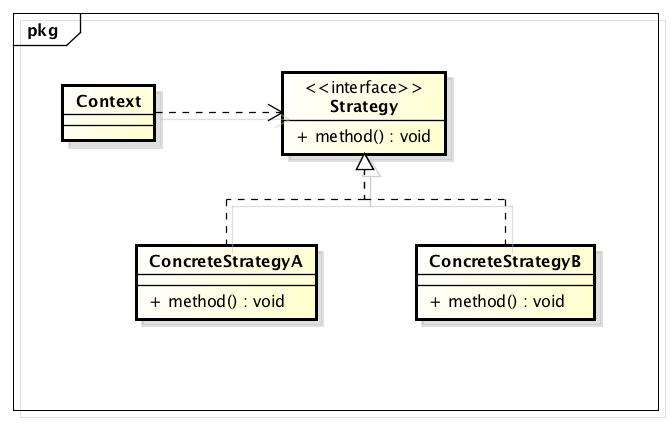
\includegraphics{../figures/strategy.png}  
  \caption{The Strategy pattern}
  \label{fig:strategy}
\end{figure}

\begin{figure}
  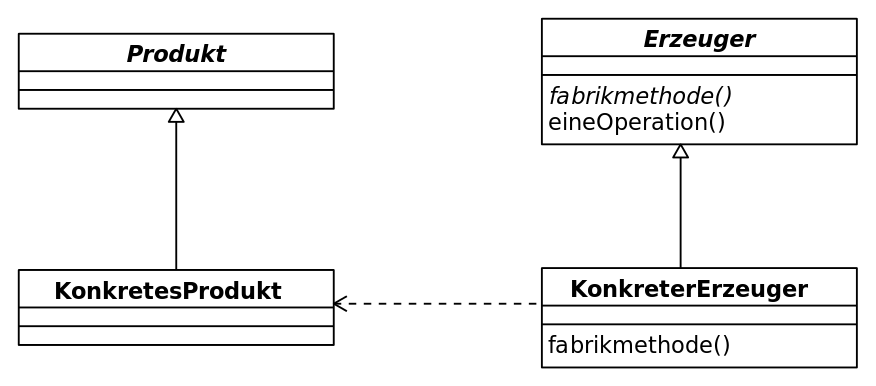
\includegraphics{../figures/factory.png}  
  \caption{The Factory pattern}
  \label{fig:factory}
\end{figure}

\begin{figure}
  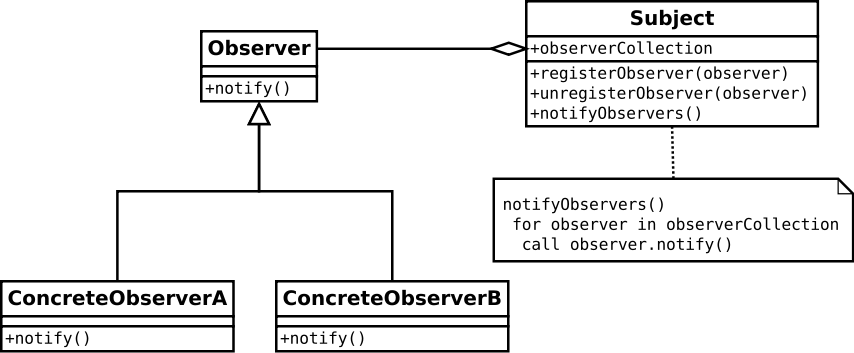
\includegraphics{../figures/observer.png}  
  \caption{The Observer pattern}
  \label{fig:observer}
\end{figure}

\begin{figure}
  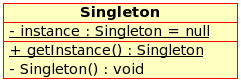
\includegraphics{../figures/singelton.png}  
  \caption{The Singelton pattern}
  \label{fig:singelton}
\end{figure}

\begin{figure}
  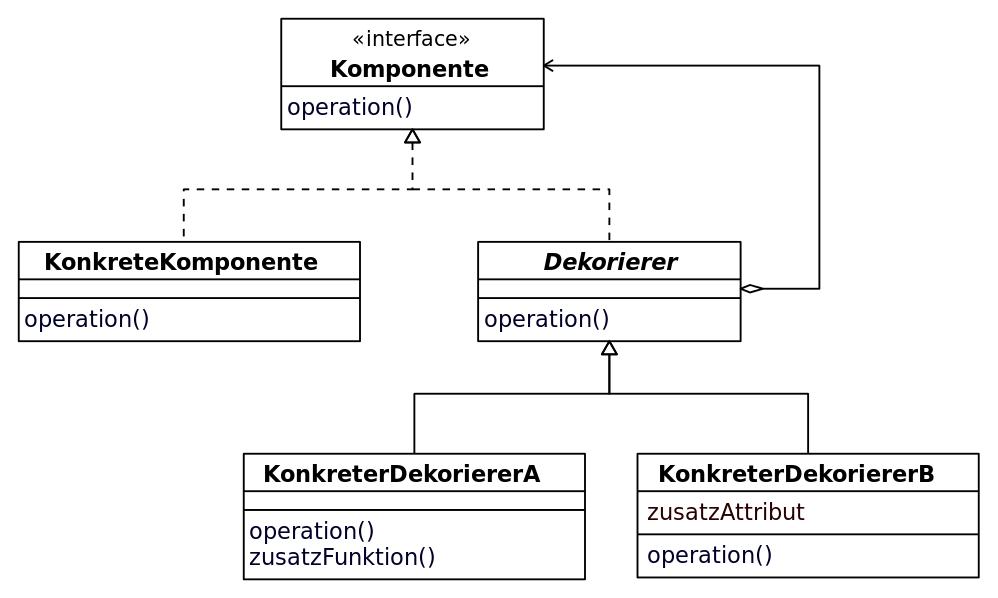
\includegraphics{../figures/decorator.png}  
  \caption{The Decorator pattern}
  \label{fig:decorator}
\end{figure}


% TODO: do more

\end{document}

